\chapter {Produktfunktionen}

\subsection{Grundfunktionalität}
\setcounter{counterKriterien}{0}
%ist noch nicht sortiert, die subsubsection kann man später wieder auskommentieren
%\subsubsection{Graphische Bedienoberfläche}
% finde es unsinnig pauschal eine Projekterstellungssicht anzuzeigen, vlcht möchte der Benutzer ein
% bereits vorhandenes Projekt öffnen. Das ist mein Vorschlag:
\nItem{PF} Startbildschirm \\
Nach dem Start der Anwendung werden dem Benutzer die zuletzt geöffneten Projekte angezeigt. Der Benutzer
hat dann die Möglichkeit ein bereits bestehendes Projekt zu öffnen oder aber ein neues Anzulegen.
%\nItem{PF} Willkommensbildschirm
%\newline
%Beim Start zeigt die Anwendung einen Willkommensbildschirm an, auf dem allgemeine Informationen und zuletzt
% benutzte Projekte zusammen mit einer \emph{Projekt-Erstellung-Sicht} angezeigt werden.
 % % % % % % % % % % % % % % % % % % % % % % % % % % % % % % % % % % % % % % % % % % % % % % % % % %
 
% Es ist unsinnig zwischen Filtern und Testsignalen zu unterscheiden. Wie soll ein Testsignal aussehen ?
\nItem{PF} Filtercontainer \\
Der Filtercontainer ist die Stelle der Grafischen Oberfläche, an der der Nutzer einen, der Anwendung
zur Verfügung stehenden, Filter auswählen kann (durch einen Klick mit der Maus). Um einen Filter auszuwählen
muss ein gültiges Video im Projektexplorer gewählt worden sein. Durch die Auswahl eines Filters wird
der entsprechende Filter als der nächste anzuwendende Filter markiert. Im Visualisierungsbereich des
Fensters kann der Nutzer alle, in der von ihm gewählten Reihenfolge, markierten Filter und auch den
dadurch verursachten Effekt sehen. Dem Benutzer steht die Möglichkeit offen einen bereits gewählten
Filter wieder abzuwählen.
% Man sollte wahrscheinlich erwähnen, dass es nicht möglich sein wird das Video abzuspielen bis der Filter 
% tatsächlich angewandt wurde.
%\nItem{PF} Testsignalansicht
%\newline
%Alle Filter und Testsignale, mit denen eine Referenzdatei manipuliert werden kann, werden aufgelistet. Der
% Benutzer kann beliebige Filter auswählen und nacheinander über einen Button auf eine (im Projektexplorer)
% bestehende Datei anwenden.
% % % % % % % % % % % % % % % % % % % % % % % % % % % % % % % % % % % % % % % % % % % % % % % % % % %

%  Wieder eine in meinen Augen nicht zielführende Unterscheidung zwischen Typen von Videos. 
%  Eine vlcht. geschicktere Version:
\nItem{PF} Projektexplorer \\
Nachdem ein bestehendes Projekt geöffnet oder ein neues erstellt worden ist wird dem
Benutzer, unter anderem, ein Projektexplorer zur Verfügung gestellt. Ein Projektexplorer ist ein 
Fenster das zwei Registerreiter enthält. \\
Der erste Reiter, die \emph{Smartlist}, enthält die dem Projekt zugewiesenen Videosequenzen. Dabei wird
grundsätzlich zwischen einer Referenz- und Erzeugten Sequenz unterschieden. Wie in Abb.\ref{pExplorer}
ersichtlich, ist die Smartlist eine Baumstruktur, dabei ist jedes Vaterelement
ein Referenzvideo im Bezug zu seinen Kindelementen. Beispielsweise ist, in Abb.\ref{pExplorer}, 
">Carphone.yuv"< ein Referenzvideo im Bezug zum Kindelement ">Gaussian Blurr"<. Gaussian Blurr ist ein
vom Nutzer gewählter Name für die Videosequenz ">Carphone.yuv"< an der der Gaußscher Weichzeichner angewandt
wurde und ">processed"< ist der vom Nutzer gewählter Name für die ">Gaussian Blurr"< Videosequenz auf
der er sein \gls{VBW} ausgeführt hat. Jede der in der \emph{Smartlist} aufgeführten wird im Projektordner
oder in einem vom Benutzer angegebenen Stelle seiner Festplatte abgelegt.\\
Der zweite Reiter \emph{Dateiexplorer} stellt eine Schnittstelle zum Dateisystem des Benutzers dar. Mit Hilfe
des Dateiexplorers kann der Nutzer \projektTitel neue Videosequenzen bekannt machen.
\begin{figure}[h]
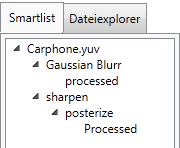
\includegraphics[scale=1]{bilder/projektexplorer.png}
\caption{Projektexplorer}
\label{pExplorer}
\end{figure}
%\nItem{PF} Projektexplorer
%\newline
%Die Anwendung listet alle Referenzvideos und Testvideos des Projekts in einem Projektexplorer auf. Der
% Benutzer kann ein oder mehrere Videos auswählen um auf diesen Filter oder Analysen auszuführen.
% % % % % % % % % % % % % % % % % % % % % % % % % % % % % % % % % % % % % % % % % % % % % % % % % % % % %
%Das ist durch die nächste PF genauer erläutert
%\nItem{PF} Darstellung der Analyseergebnisse als Diagramme
%\newline
%Die Analysedaten werden nach Möglichkeit graphisch durch z.B. Diagramme dargestellt.
% Im Prinzip nicht(komplett ;-) ) falsch, aber die Formulierung gefählt mir nicht und außerdem würden
% wir uns dadurch auf nur eine Art der Visualisierung festlegen.
%\nItem{PF} Darstellung der Analyseergebnisse als Overlay
%\newline
%Analysedaten (z.B. berechnete Unterschiede) werden als Overlay über dem Video eingeblendet.
% Hier eine Alternative
% edit: habe meine Alternative nun auskommentiert da ein paar Zeilen weiter das gleiche in einem 
% besseren Zusammenhang erklärt wird
%\nItem{PF} Die Ergebnisse eines Analysevorgangs werden im Visualisierungsbereich von \gls{OQAT} dargestellt.
%Die Art der Darstellung hängt dabei von der gewählten Analysemetrik ab. Wenn z.B. \gls{mse} als die
%zu verwendende Analysemetrik gewählt wurde wird neben des Differenzvideos(wobei ein Pixel den \gls{mse}
%Wert des jeweiligen Pixels trägt) auch der globale \gls{mse} für das jeweilige Frame und für die gesamte
%Videosequenz dargestellt.
%\nItem{PF} GUI
%\newline
%Die Anwendung unterstützt eine interaktive graphische Benutzeroberfläche mit verschiedenen Sichten, die ein-
% und ausgeblendet werden können. Dabei können Ein- und Ausgabevideos abgespielt, sowie einzelne Frames
%  ausgewählt und visuallisiert werden.
\nItem{PF} Graphische Oberfläche \\
\gls{OQAT} stellt dem Nutzer eine Interaktive Benutzeroberfläche zur Verfügung, die
einzelnen Bestandteile dieser werden im Kapitel \emph{Graphische Oberfläche} näher erläutert.\\
% Gleiches Argument wie oben, das Zeug ist noch nicht sortiert. Da sind pseudoKapitel nur verwirrend.
%\subsubsection{Projektverwaltung}
% Etwas ungenau, sowas haben wir bereits in dem MK. An dieser Stelle muss man also etwas spezifiescher
% werden
%\nItem{PF} Projektverwaltung
%\newline
%Die Anwendung bietet dem Benutzer die Möglichkeit, durch eine \emph{Projekt-Erstellung-Sicht} Projekte
% anlegen, speichern, löschen und verwalten zu können.
\nItem{PF} Projekte anlegen \\
Um \gls{OQAT} verwenden zu können muss der Benutzer ein neues Projekt anlegen oder aber
ein bereits existierendes öffnen. \\
Ein neues Projekt kann entweder über das Hauptmenü, Toolbar oder aber mit Hilfe des sich
im Startfensters befindenden Buttons angelegt werden. Nachdem der Nutzer eine dieser Möglichkeiten
in Anspruch genommen hat, öffnet sich Projekterstellungs-Dialog. In diesem Dialog
muss der Benutzer folgende Daten angeben:
\begin{compactitem}
\item Projektname
\item Ein Pfad unter dem die Projektdaten abgelegt werden sollen. Dieses kann auch leer gelassen werden, 
dann wird ein Defaultpfad verwendet.
\end{compactitem}
% Diese Funktionalität ist in der ">ProjektExplorer"< etwas genauer erläutert worden
%\nItem{PF} Laden von Referenzdateien
%\newline
%Der Benutzer kann durch ein Dialogfenster eine Referenzdatei im YUV-Format in ein Projekt laden, indem er
% den Pfad zu der Datei angibt. Es können mehrere Referenzdateien geladen werden.

%\subsubsection{Portabilität}
%
%\subsubsection{Analyse}

%\nItem{PF} Analysewerkzeugsicht
%\newline
%Alle verfügbaren Analysewerkzeuge werden in dieser Sicht aufgelistet. Der Benutzer kann beliebige Werkzeuge
% markieren und schließlich über einen Button einen Analysedurchlauf für die aus dem Projektexplorer
%  ausgewählten Videodateien starten.
\nItem{PF} MetriList\\
Die \emph{MetriList} enthält alle der Anwendung zur Verfügung stehenden Analysemetriken.
Sobald im SmartTree ein Video und ein gültiges Referenzvideo ausgewählt wurde, darf der Benutzer
eine oder mehrere Metriken auswählen. Eine erfolgreiche Auswahl wird durch das hervorheben des
jeweiligen Eintrags der \emph{MetriList} und einen entsprechenden Vermerk in dem Visualisierungsbereich
gekennzeichnet. Eine Metrik kann erst ausgewählt werden wenn möglicherweise zuvor gewählte Filter,
z.B. durch den Klick auf das entsprechende Symbol aus der Toolbar, bereits angewandt wurden. Versucht
der Benutzer eine Metrik auszuwählen ohne ein Video und Referenzvideo entsprechend markiert zu haben oder
während markierte aber nicht abgearbeitete Filter existieren wird er darauf hingewiesen.

% Muss es hier hin ? In den Musskriterien ist das gleiche drin. -> entweder hier genauer oder aber
% unnötig
%\nItem{PF} Analyse-Metriken
%\newline
%\projektTitel stellt dem Benutzer einige Analyse-Metriken standardmäßig bereit:
%\begin{itemize}
%\item \gls{MSE}
%\item \gls{PSNR}
%\end{itemize}

% Ziemlich wage Formulierung. 
%">..Video werden anhand einer Metrik verglichen.."< Wie genau soll das aussehen ?
%"<..Ergebnisse werden analysiert"< achja ? Wozu und vorallem wie sollen wir die Ergebnisse analysieren ?
% Die Auswertung der Ergebnisse überlassen wir dem Benutzer, wir errechnen die Ergebnisse anhand einer
% Metrik, nicht mehr und nicht weniger. Die Logdatei speichern Geschichte gehört hier nicht ganz hin,
% schließlich hat der Nutzer auch die Möglichkeit solche Daten auch nach dem Durchlauf(nächste Woche..)
% zu exportieren -> Es ist eine eigene Funktionseinheit die beschrieben werden sollte.
% 
%\nItem{PF} Analysedurchlauf
%\newline
%Wenn ein Analysedurchlauf gestartet wird, werden die ausgewählten Videos mittels der ausgewählten
% Analysemetriken verglichen und die Ergebnisse analysiert, bewertet und optional in eine Logdatei
%  gespeichert. Dem Nutzer werden während des Analysedurchlaufs ein Fortschrittsbalken und Statusmeldungen
%   angezeigt. 
% hier ein Gegenvorschlag:
\nItem{PF} Analysevorgang \\
Nachdem der Nutzer eine oder mehrere Metriken aus der \emph{MetriList} und ein
Video samt einem Referenzvideo ausgewählt hat, kann der Benutzer einen Analysevorgang starten. Hat der
Nutzer mehrere Metriken ausgewählt werden diese im Batchverfahren abgearbeitet. Nachdem ein Analysevorgang
beendet wurde, stehen dem Nutzer die Ergebnisse im Visualisierungsbereich zur Verfügung(wurden 
mehrere Metriken angewandt werden diese unter verschiedenen Registerreitern des Visualisierungsbereichs
abgelegt). Die Art der Darstellung der Analyseergebnisse hängt ganz und gar von der Art der gewählten 
Metrik ab. Wenn Beispielsweise die Metrik gls{mse} gewählt wurde wird neben des Differenzvideos(wobei ein
Pixel den \gls{mse} Wert des jeweiligen Pixels trägt) auch der globale \gls{mse} für das jeweilige Frame
und für die gesamte Videosequenz dargestellt.
%%%%%%%%%%%%%%%%%%%%%%%%%%%%%%%%%%%%%%%%%%%%%%%%%%%%%%%%%%%%%%%%%%%%%%%%%%%%%%%%%%%%%%%%%%%%%%%%%%%%%
% ist noch nicht sortiert
%\subsubsection{Verzerrung}
% Eine detailiertere Version davon ist unter PF Filtercontainer zu finden
%\nItem{PF} Filter
%\newline
%Ein Video, welches in ein Projekt eingebunden wurde, kann durch Filter verzerrt werden.Dieses wird
%nach dem Verzerren mit ihrem Referenzvideo verknüpft  Auf solch ein verzerrtes Video kann über den Projektexplorer zugegriffen werden um es ggf. weiter zu verzerren oder zu analysieren.


% Unsinnige unterscheidung zwischen Testsignalen und Filtern
% Das mit den externen Filtern ist eine haarige Angelegenheit
\nItem{PF} Filter-Plugins
\newline
Die Anwendung ist um beliebige Testsignale und Filter in der Form von Plugins erweiterbar.
 Videobearbeitungswerkzeuge (wie z. B. Encoder) kann man auch als externe Filter betrachten und sie als
  Plugins laden, solange sie die Form von ausführbaren Programmen haben und über die Kommandozeile 
angesteuert werden können.

% Bin mir nicht sicher ob es hier nochmal aufgegriffen werden muss
% Bei den Musskriterien ist eine etwas treffendere Beschreibung drin.
% Welchen Zweck wird kantendetektion haben ?
\nItem{PF} Standard-Filter
\newline
Die Anwendung stellt dem Benutzer einige Filter standardmäßig bereit:
\begin{itemize}
\item Weichzeichner
\item Rauschen
\item Farbfilter
\item Blur
\item Schärfe
\item Kantendetektion
\item Emboss
\item Dilatation (Erweiterung)
\item Erosion (Abtragung)

\end{itemize}
%  Etwas kurz geraten, weiter unten ist meine Version
%\nItem{PF} Generierung von Testdateien
%\newline
%Wendet man ausgewählte Filter auf eine Datei an, dann wird eine durch die jeweiligen Filter manipulierte Datei im \gls{glos:YUV} Format generiert, die im Projektordner gespeichert und im Projektexplorer bei den Testvideos aufgelistet wird.
\nItem{PF} Filtervorgang\\
Nachdem der Nutzer einen oder mehrere Filter, gemäß der PF Filtercontainer, markiert hat, kann er
den Filtervorgang, durch den Klick auf das entsprechende Symbol in der Toolbar oder im Hauptmenü,
einleiten. Die Dauer des Filtervorgangs ist Abhängig von der Anzahl der gewählten Filter und der Auflösung
und Länge des gewählten Video aus der Smartlist. Nach einem Filtervorgang wird das neu entstandene Video
als Kindelement, des für den Filtervorgang ausgewähltem Video, aufgeführt.

\subsection{Optionale Funktionalität}
\nItem{PF} Motion Vektoren des .H264 Encoders des \gls{ITEC}\\
Der .H264 Encoder des Instituts gibt, neben der encodierten Videosequenz, auch die verwendeten Motion
Vektoren. \gls{OQAT} kann diese Vektoren im Visualisierungsbereich darstellen.\\
nItem{PF} Drag and Drop\\
Der Projektexplorer ist \emph{Drag and Drop} fähig, d.h. eine gültige Videodatei kann nicht nur über
die Toolbar oder das Hauptmenü hinzugefügt werden sondern darf auch nach dem \emph{Drag and Drop} Prinzip
in die Smartlist eingefügt werden. Das einzubindende Video kann dabei als ein neues Element (ohne
Vaterelement) oder aber als Kindelement eines bereits vorhandenen Videos eingefügt werden.
% So ziehmlich das gleiche ist in unseren WKs zu finden.
%\nItem{PF} Vorschau für Filter
%\newline
%Die Auswirkungen eines Filters oder Testsignals auf ein gewähltes Video werden dem Benutzer als Vorschau an einem Frame veranschaulicht.
% Ich dachte wir haben uns davon verabschiedet.
%
%\nItem{PF} Eingebaute Kommandozeile
%\newline
%Der Benutzer hat die Möglichkeit, durch eine Kommandozeile Argumente an die Anwendung übergeben zu können.
% Eine ähnliche Beschreibung ist in den Musskriterien verzeichnet
%\nItem{PF} Logdatei
%\newline
%Es gibt die Option, eine Logdatei für einen Analysevorgang zu erstellen. In der Logdatei sollen im Rahmen
% des jeweiligen Analysevorgangs ausgeführte Operationen sowie erhaltene Ergebnisse in Textformat
%  chronologisch aufgelistet werden. Die Auswahl, welche Arten von Operationen und Ergebnissen in der
%   Logdatei gespeichert werden sollen, steht dem Benutzer zur Verfügung.


